\documentclass[a4paper]{article}
\usepackage{geometry}
\usepackage{amsmath, amssymb, amsthm}
\usepackage{algorithm}
\usepackage{algpseudocode}
\usepackage{booktabs}
\usepackage{xcolor}
\usepackage{listings}
\usepackage{hyperref}
\usepackage{tikz}
\lstset{
    basicstyle=\ttfamily\small,
    keywordstyle=\color{blue}\bfseries,
    commentstyle=\color{green!50!black}\itshape,
    stringstyle=\rmfamily\upshape,
    numbers=left,
    numberstyle=\tiny\color{gray},
    stepnumber=1,
    numbersep=5pt,
    backgroundcolor=\color{white},
    showstringspaces=false,
    breaklines=true,
    frame=single,
    rulecolor=\color{black},
}

\theoremstyle{definition}
\newtheorem{lemma}{Lemma}
\newtheorem{theorem}{Theorem}
\newtheorem{remark}{Remark}

\title{\bf{Opimizing SPFA via Tarjan's Subtree Disassembly Trick}}
\author{Yanqiao Chen\\
        Southern University of Science and Technology\\
        Department of Computer Science and Engineering\\
        \texttt{12412115@mail.sustech.edu.cn}}
\date{\today}

\begin{document}

\maketitle

\section{Tarjan's Subtree Disassembly Trick}

\subsection{Observation: Why it works, intuitively?}

Tarjan's Subtree Disassembly Trick\cite{shokry2019shortestpathalgorithmstheory} is a useful technique for optimizing the Shortest Path Faster Algorithm (SPFA) by decomposing the graph into subtrees. Each node in the graph preserves a pointer to its parent node, and thus it forms a tree structure that represents the shortest paths.

Each time when we need to relax an edge $(u, v)$, we immediately find $u$ in the subtree of $v$ instead of backtracking. Once we found $u$, it means that there exists a negative cycle. 

If there is no negative cycle, we delete the whole subtree of $v$ and annotate all the nodes as not discovered and pop them out of the queue. This is because now the estimation base on the new $d(v)$, thus all the estimation made by the previous $d(v)$ is invalid.

The algorithm made very clever pruning method: First, the algorithm will look ahead whether the node in the queue is useful or not. If a $v$ is updated frequently, then nodes will be in-queued frequently, leading to a efficiency degradation.

\subsection{Pseudocode}

For comparison, we first list the standard SPFA in Algorithm~\ref{alg:spfa-standard}. The Tarjan-optimized version is given in Algorithm~\ref{alg:spfa-tarjan}.

We provide the auxiliary function in Algorithm~\ref{alg:is-in-subtree} and Algorithm~\ref{alg:delete-subtree} to preserve the subtree structure.

\begin{algorithm}[H]
\caption{Standard SPFA}
\label{alg:spfa-standard}
\begin{algorithmic}[1]
\Require Graph $G = (V, E)$, source node $s$
\Ensure Distance array $d$, or report a negative cycle
\State Initialize $d[v] \gets +\infty$, $\text{count}[v] \gets 0$, $\text{inqueue}[v] \gets \text{false}$ for all $v \in V$
\State $d[s] \gets 0$
\State $Q \gets \text{Queue}(\{s\})$, $\text{inqueue}[s] \gets \text{true}$
\While{$Q$ is not empty}
    \State $u \gets Q.\text{dequeue}()$
    \State $\text{inqueue}[u] \gets \text{false}$
    \For{each edge $(u, v)$ with weight $w$}
        \If{$d[u] + w < d[v]$}
            \State $d[v] \gets d[u] + w$
            \If{$\neg\,\text{inqueue}[v]$}
                \State $Q.\text{enqueue}(v)$
                \State $\text{inqueue}[v] \gets \text{true}$
                \State $\text{count}[v] \gets \text{count}[v] + 1$
                \If{$\text{count}[v] > |V|$}
                    \State \Return ``Negative cycle detected''
                \EndIf
            \EndIf
        \EndIf
    \EndFor
\EndWhile
\State \Return $d$
\end{algorithmic}
\end{algorithm}

\begin{algorithm}[H]
\caption{Auxiliary Procedure: \textsc{Is-In-Subtree}$(u, v)$}
\label{alg:is-in-subtree}
\begin{algorithmic}[1]
\Function{Is-In-Subtree}{$u, v$}
    \State $\text{curr} \gets v$
    \While{$\text{curr} \neq \text{null}$}
        \If{$\text{curr} = u$}
            \State \Return \textbf{true}
        \EndIf
        \State $\text{curr} \gets \text{parent}[\text{curr}]$
    \EndWhile
    \State \Return \textbf{false}
\EndFunction
\end{algorithmic}
\end{algorithm}

\begin{algorithm}[H]
\caption{Auxiliary Procedure: \textsc{Delete-Subtree}$(x)$}
\label{alg:delete-subtree}
\begin{algorithmic}[1]
\Function{Delete-Subtree}{$x$}
    \State $S \gets \text{Stack}(\text{children}[x])$
    \State $\text{children}[x] \gets \emptyset$
    \While{$S$ is not empty}
        \State $y \gets S.\text{pop}()$
        \State $d[y] \gets +\infty$
        \State $\text{inqueue}[y] \gets \text{false}$
        \State $\text{parent}[y] \gets \text{null}$
        \For{each $z \in \text{children}[y]$}
            \State $S.\text{push}(z)$
        \EndFor
        \State $\text{children}[y] \gets \emptyset$
    \EndWhile
\EndFunction
\end{algorithmic}
\end{algorithm}

\begin{algorithm}[H]
\caption{SPFA with Tarjan's Subtree Disassembly Trick}
\label{alg:spfa-tarjan}
\begin{algorithmic}[1]
\Require Graph $G = (V, E)$, source node $s$
\Ensure Distance array $d$, or report a negative cycle
\State Initialize $d[v] \gets +\infty$, $\text{parent}[v] \gets \text{null}$, $\text{children}[v] \gets \emptyset$, $\text{inqueue}[v] \gets \text{false}$ for all $v \in V$
\State $d[s] \gets 0$
\State $Q \gets \text{Queue}(\{s\})$, $\text{inqueue}[s] \gets \text{true}$
\While{$Q$ is not empty}
    \State $u \gets Q.\text{dequeue}()$
    \State $\text{inqueue}[u] \gets \text{false}$
    \For{each edge $(u, v)$ with weight $w$}
        \If{$d[u] + w < d[v]$}
            \If{\Call{Is-In-Subtree}{$u, v$}}
                \State \Return ``Negative cycle detected''
            \EndIf
            \State \Call{Delete-Subtree}{$v$}
            \If{$\text{parent}[v] \neq \text{null}$}
                \State $\text{children}[\text{parent}[v]].\text{remove}(v)$
            \EndIf
            \State $\text{parent}[v] \gets u$
            \State $\text{children}[u].\text{add}(v)$
            \State $d[v] \gets d[u] + w$
            \If{$\neg\,\text{inqueue}[v]$}
                \State $Q.\text{enqueue}(v)$
                \State $\text{inqueue}[v] \gets \text{true}$
            \EndIf
        \EndIf
    \EndFor
\EndWhile
\State \Return $d$
\end{algorithmic}
\end{algorithm}


\subsection{What makes it different: The key idea of Tarjan's trick} 

Let us consider a bottleneck in standard SPFA. Suppose node $u$ is dequeued and relaxes an edge to its neighbor $v$, yielding a smaller $d[v]$. Node $v$ is then enqueued. However, if $v$ already had a subtree of descendants in the current shortest-path tree, those descendants retain distance estimates derived from the obsolete value of $d[v]$. They may still reside in the queue (or be processed later through other updates) and continue propagating those stale values, causing redundant relaxations. When $v$ has a large subtree, this waste becomes severe.

Tarjan's Subtree Disassembly Trick eliminates this inefficiency immediately. As soon as $v$'s distance is updated, the algorithm invokes $\textsc{Delete-Subtree}(v)$: it traverses $v$'s entire old subtree, resets every descendant's distance to $+\infty$, clears their parent pointers, removes them from the queue if present, and discards their child lists. Only after this aggressive pruning is $v$ linked to its new parent $u$ and enqueued. By tearing down the obsolete subtree instantly, the trick ensures that no node ever propagates a stale distance estimate, which drastically reduces the number of useless relaxations. 

This idea can be seen as a form of eager pruning. In the shortest-path tree maintained by the algorithm, every descendant's distance is inductively derived from its ancestors: each node's estimate equals the total edge weight along the unique tree path from the source. Thus the validity of the entire subtree is contingent on the root's distance remaining unchanged. The instant $d[v]$ is updated, all prior estimates in $v$'s subtree become obsolete. Instead of letting these stale values linger in the queue and trigger useless relaxations, the algorithm discards the subtree immediately. This ensures that every pending relaxation is grounded in a fresh, valid distance estimate.

\section{The Complexity Analysis}

\subsection{Amortized Analysis}

We analyze the amortized cost of a successful relaxation. In $\textsc{Delete-Subtree}(v)$, every node in the old subtree rooted at $v$ is visited a constant number of times (popped from the stack, reset, and its children are pushed). Thus the actual cost of deleting a subtree of size $s$ is at most $c \cdot s$ for some fixed constant $c \geq 1$.

We use the potential method with
\[
    \Phi = c \cdot (\text{total number of nodes currently in the shortest-path tree}).
\]
Equivalently, $\Phi = c \cdot \sum_{v \in V} |\text{children}[v]|$.

Consider a successful relaxation of edge $(u,v)$. Let $s$ be the size of the old subtree rooted at $v$.
\begin{itemize}
    \item \textbf{Delete-Subtree:} The actual cost is at most $c \cdot s$. The subtree is removed from the tree, so the potential drops by $c \cdot s$.
    \item \textbf{Re-attach $v$:} The actual cost is $O(1)$. Node $v$ is added as a child of $u$, so the potential increases by $c$.
\end{itemize}

The net change in potential is $\Delta\Phi = -c \cdot s + c$. Therefore the amortized cost is
\[
    \hat{c} = c_{\text{actual}} + \Delta\Phi \leq (c \cdot s + O(1)) + (-c \cdot s + c) = O(1).
\]

Thus every successful relaxation has $O(1)$ amortized cost. Since each node's distance can be updated at most $O(|V|)$ times in a graph with no negative cycles, the number of successful relaxations is $O(|V| \cdot |E|)$, and the total amortized cost of all successful relaxations is $O(|V| \cdot |E|)$. The practical gain of Tarjan's trick comes from eliminating useless relaxations by stale nodes, not from improving the asymptotic worst-case bound.

The worst case follows the amortized complexity, which is also $O(|V|\cdot |E|)$.

\subsection{Space Complexity} 

The complexity of this algorithm is simple. We only have to preserve a double direction link list ($O(n)$) for the tree, the adjacent list ($O(m)$) and other auxiliary arrays (distance, and a queue, $O(n)$). Thus the total space complexity is $O(m + n)$.

\section{In what case do the new algorithm performs better} 

Let us construct a simple case such that the SPFA degrades.

\textbf{Graph construction.} Consider the graph $G$ illustrated in Figure~\ref{fig:degenerate-case}. It contains a source $s$, an intermediate node $a$, a hub node $h$, and $n$ leaf nodes $\ell_1, \dots, \ell_n$. The edge weights are chosen so that $h$ is first reached via the direct edge $s \to h$ with distance $0$, and later via the detour $s \to a \to h$ with a strictly smaller distance $-5$. Every leaf $\ell_i$ is attached to $h$ with weight $0$.

\begin{figure}[H]
\centering
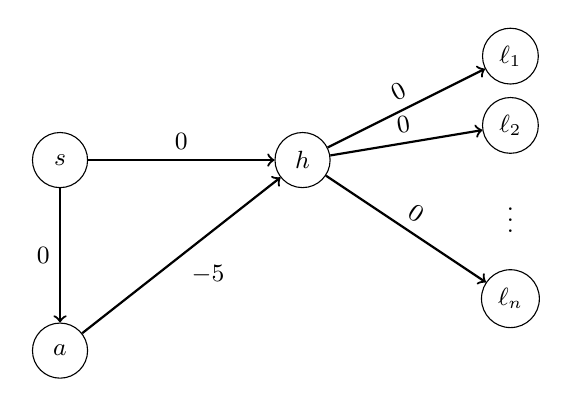
\begin{tikzpicture}[scale=1.1, every node/.style={font=\small}]
    \tikzset{vertex/.style={circle, draw, minimum size=7mm}}

    \node[vertex] (s) at (0,0) {$s$};
    \node[vertex] (a) at (0,-2.2) {$a$};
    \node[vertex] (h) at (2.8,0) {$h$};

    \node[vertex] (l1) at (5.2, 1.2) {$\ell_1$};
    \node[vertex] (l2) at (5.2, 0.4) {$\ell_2$};
    \node (ld) at (5.2,-0.6) {$\vdots$};
    \node[vertex] (ln) at (5.2,-1.6) {$\ell_n$};

    \draw[->, thick] (s) -- (h) node[midway, above] {$0$};
    \draw[->, thick] (s) -- (a) node[midway, left] {$0$};
    \draw[->, thick] (a) -- (h) node[midway, below right] {$-5$};

    \foreach \dest in {l1,l2,ln} {
        \draw[->, thick] (h) -- (\dest) node[midway, above, sloped] {$0$};
    }
\end{tikzpicture}
\caption{A degenerate case for standard SPFA. For simplicity, the node $h$ represents a node that will be frequently updated, while the number of the downstream nodes is large. We will not draw the complete graph for simplicity.}
\label{fig:degenerate-case}
\end{figure}

This star-shaped structure is deliberately simple; the key is to imagine that each leaf $\ell_i$ is the entry point to a downstream subgraph (a chain, a tree, or a dense component). The downstream structure is omitted from the figure for clarity, but it is where the inefficiency manifests.

When $h$ is relaxed, all its descendants are enqueued for subsequent processing. If $h$ is relaxed again later, a new batch of descendants is enqueued with improved distances, while the previous copies---still residing in the queue---continue to carry stale estimates. These obsolete nodes then propagate incorrect information through their downstream subgraphs, causing cascading redundant work. Tarjan's Subtree Disassembly Trick avoids this entirely by deleting the entire obsolete subtree the moment $h$ is updated, pruning all stale descendants before they can perform any useless relaxations.

This example demonstrates that the gain of Tarjan's Subtree Disassembly Trick is not a better asymptotic bound, but the elimination of massive redundant work by eagerly invalidating stale subtrees before they can cascade. 

\begin{remark}
When the graph contains a negative cycle, Tarjan's algorithm detects it via $\textsc{Is-In-Subtree}(u, v)$, which traverses only the ancestors of $v$ in the current shortest-path tree. Standard SPFA, by contrast, relies on counting enqueue operations ($\text{count}[v] > |V|$) and may require up to $O(|V|)$ updates per node before detection. In practice, the Tarjan version can discover negative cycles earlier because the check is performed immediately upon relaxation rather than after a threshold is reached. This is a modest but tangible efficiency improvement. However, both algorithm can be hack by specific graph, thus the worst case complexity won't change.
\end{remark}

\section{Conclusion} 

Tarjan's Subtree Disassembly Trick is a pragmatic heuristic for SPFA. It does not improve the asymptotic worst-case or amortized complexity; the theoretical bound remains $O(|V| \cdot |E|)$. The practical gain comes from eliminating cascading useless relaxations, not from a smaller constant factor. There is an inherent trade-off: every successful relaxation pays an additional $O(s)$ cost for $\textsc{Delete-Subtree}$ (where $s$ is the size of the obsolete subtree), but in return it avoids $\Theta(s \cdot \bar{w})$ wasted work that stale nodes would otherwise inflict on their downstream subgraphs. This trade-off is favorable on graphs where nodes are updated frequently or possess large subtrees, which explains why the Tarjan-optimized variant often outperforms standard SPFA in practice. 



\bibliographystyle{plain}
\bibliography{references}

\end{document}
